% 23 jan 2012  jh: add new formats
%  2 feb 2012  lo: add comment on version of GSE
% 27 nov 2012  jh: small change on time
% 05 dec 2012  jh: more on cont bases
% 28 dec 2012  jh: use of sample_wav_read to make archive channels
% 09 jan 2013  jh: more ARC description
%\chapter{STRUCTURE OF SEISAN}
\chapter{Structure of SEISAN}
\label{chp:struc}

\section{Directories}

The whole SEISAN system is located in subdirectories residing under the main 
directory SEISMO. For more details, see %section 3 
chapter \ref{chap:installation} on installation. The system 
contains the following main subdirectories: 

\begin{tabular}{|ll|}
\hline
REA:& Earthquake readings and full epicenter solutions in a database  \\
WOR:& The users work directory, initially empty  \\
TMP &Temporal storage of files, initially empty  \\
PRO:& Programs, source code and executables  \\
LIB:& Libraries and subroutines  \\
INC:& Include files for programs and subroutines in PRO and LIB  \\
COM:& Command procedures  \\
DAT:& Default and parameter files, e.g. station coordinates  \\
WAV:& Digital waveform data files  \\
CAL:& System calibration files  \\
INF:& Documentation and information  \\
ISO:& Macroseismic information  \\
SUP:& Supplementary files and programs  \\
\hline
\end{tabular}

In the following, the above subdirectories will mostly be called directories to avoid always referring to SEISMO. All directories use capital letters, however this only makes a difference in the Unix versions. The directory structure is used as a tree like structure for quick access to individual files in the REA directory, which therefore will appear as a simple database to the user. The next section is a description of the database directories; the other directories are described in %section 7
chapter \ref{chap:programming}. Figure %1 
\ref{fig:structure} shows the tree structure of SEISAN. 

\begin{figure}
\htmlimage{scale=2.0}
%\centerline{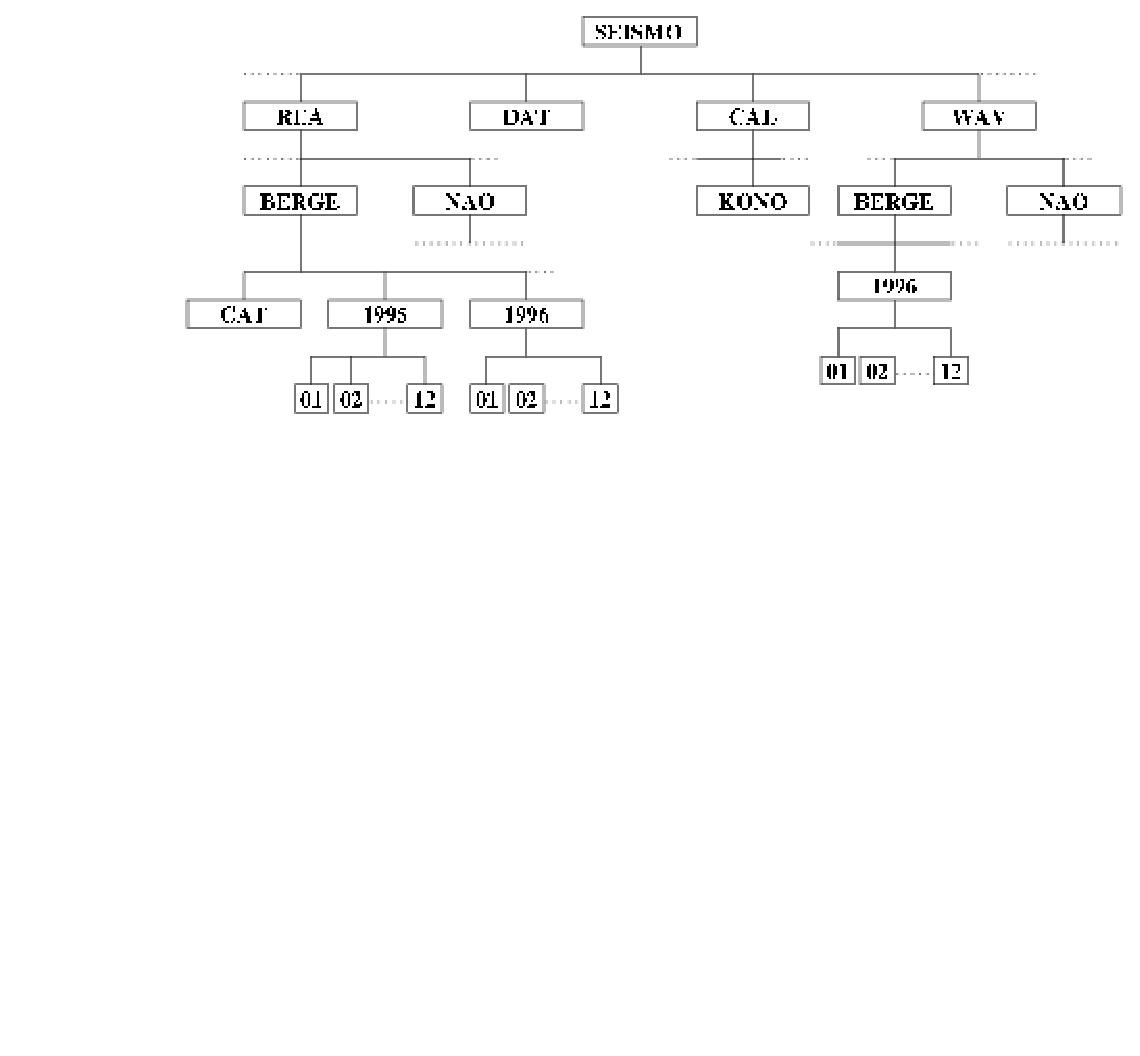
\includegraphics[width=0.9\linewidth]{fig/fig1.eps}}
\centerline{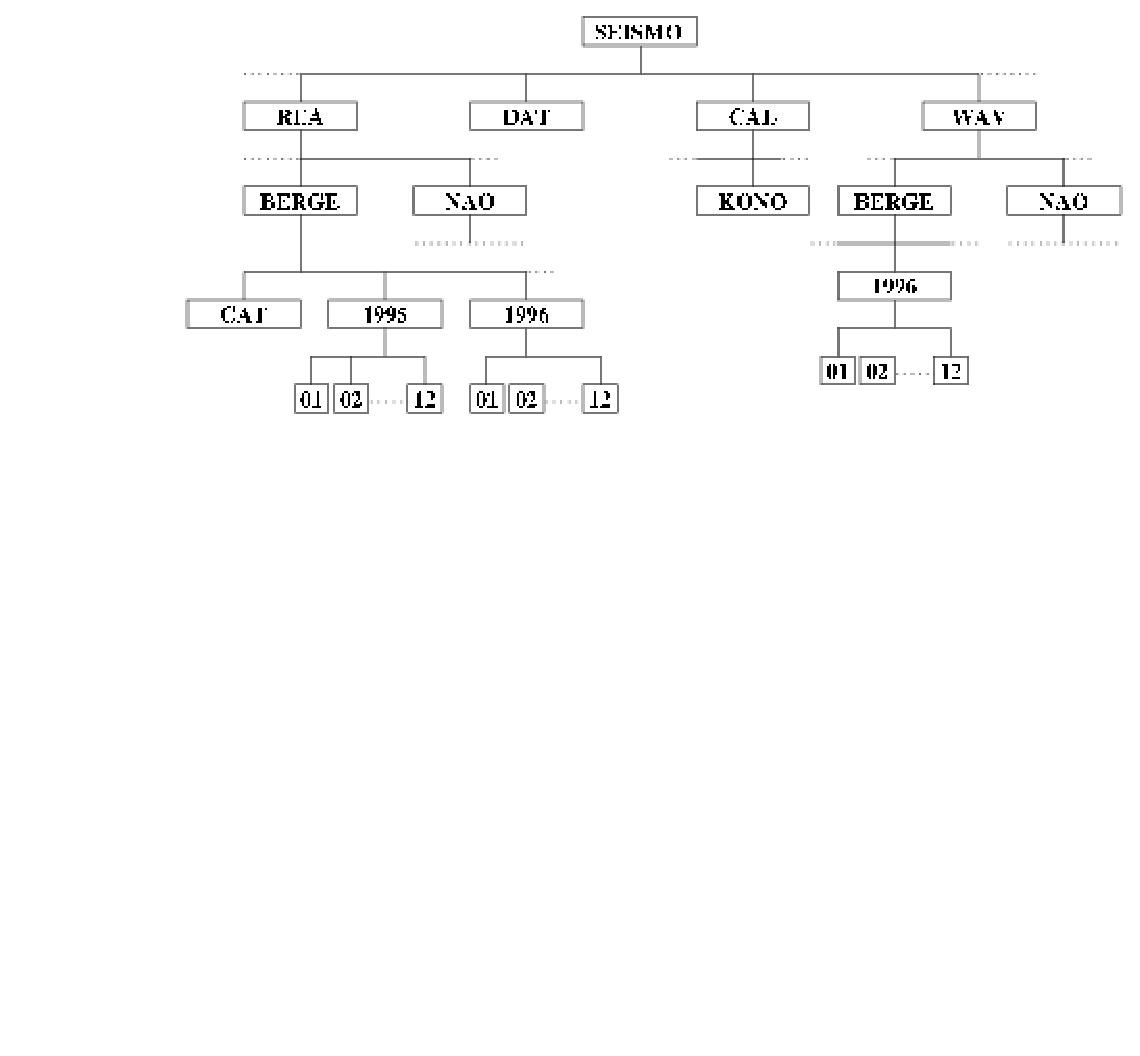
\includegraphics[width=0.9\linewidth]{fig/fig1}}
\caption{Structure of SEISAN. Note that BERGE under WAV is optional and 
DELET (not shown) under REA has a similar directory structure as e.g. NAO.}
\label{fig:structure}
\end{figure}

\section{The database}
The database of SEISAN consists of the two directories REA and WAV. 
The REA directory and its subdirectories contain readings and source 
information while all waveform data is normally in the directory WAV 
(see \ref{subs:waveform}) with no subdirectories. Optionally WAV can also be divided 
into a similar subdirectory structure, see \ref{subs:waveform}, which is useful 
when storing continuous data in particular. 
The \index{DEL directory}DELET database contains all events deleted 
from any of the databases (here BERGE/BER and NAO). Filenames are 
identical between all platforms. 

% 2.2.1 Phase data and hypocenters{tc \l 3 "2.2.1 Phase data and hypocenters, the REA directory} 
\subsection{Phase data and hypocenters}

The \index{REA directory}REA directory contains phase readings and 
derived source information like hypocenters, fault plane solutions 
etc. The REA directory has one or several subdirectories corresponding 
to separate databases (see Figure \ref{fig:structure} for an example 
with two databases). The database names can have between 3 and 5 
characters. If less than 5 characters are used, the character `\_' 
is added in the file system to make it 5. The user does not have to 
put the `\_' when running a program, they will be added by the software. 
If a directory is made manually, the `\_' must be put in. It is assumed 
that a  database is always present in the system. The name of the default 
database is given by an environmental variable (see section \ref{sect:instal-unix}), 
however if not set, it will default to \index{AGA}AGA for agency. 
Here, BER will be used as an example throughout the manual. A database 
has a duplicate storage of the events. For quick reference and interactive 
work the events are stored in \index{Single files}single files (S-files) 
in yearly directories and monthly subdirectories. When new data is 
entered into the database, it comes in as individual event files. 
However, once the interactive work has finished, the single event 
files are overwritten with the final location and additionally stored 
in monthly files, which are only changed when updating (UPDATE command, 
see section \ref{sect:update-upd}). 
The monthly files, called \index{CAT-file}CAT-files 
for catalog, are stored separately in the CAT directory and primarily 
used for quick searching and backup for the single files. In addition 
to the event data, there is also a \index{LOG directory}LOG directory 
in each database to keep a log of the data processing, 
see section \ref{sect:update-upd}. 

\textbf{S-file database structure}
\index{S-file}

The structure for the single file storage is as follows (Windows example): 

\begin{tabular}{|ll|}
\hline
\textbackslash REA\textbackslash BER\_\_\textbackslash  & Main readings directory, all data  \\
\textbackslash REA\textbackslash BER\_\_\textbackslash 1999\textbackslash & Data for 1999  \\
\textbackslash REA\textbackslash BER\_\_\textbackslash 1999\textbackslash 01\textbackslash &  Data for January 1999, each event in one file  \\
\hline
\end{tabular}

On Unix, the last line would have been /REA/BER\_\_/1999/01 

The structure works back year 0000. Each event contains original phase readings in the 
\index{Nordic format}Nordic format (
Appendix \ref{app:nordic}. 
) which includes file 
names of all corresponding waveform files. One event is one file. 
Each event has an ID line. The ID line contains a unique ID, which 
will follow the event through all COLLECT and SPLIT operations 
(see section \ref{sect:collect} and \ref{sect:split}). The \index{ID-line}ID line 
also contains status information about the event like last action, 
when it was updated etc. The ID-number can be fixed, which is useful 
if data is taken out from the database, processed on another computer and later put back into the database, since otherwise the ID of an event might be changed and the existing file would not be overwritten. An example of an S-file name is :\newline
\texttt{27-1112-11L.S199401}

The S-files are used as input for the location program and, 
when making a permanent update, also for output, see \ref{sect:hypocenter}. 
The letter in front of the "." indicates the \index{Event type}event 
type and can be L, R or D for local, regional or distant event 
respectively. It is the same indicator as given in the header line 
of the S-file, see the Nordic format page \pageref{app:nordic}. 
The remaining numbers give (in order) day, hr, min, sec, year and month.  

As mentioned above, the system can contain many 
\index{Other databases}other databases, which may function exactly 
like the BER directory. A data base can be used to store a subset 
of data or data from different networks. Data can be moved between 
databases or in and out of the databases, for details, see description 
on EEV (\ref{sect:interactive} and \ref{sect:eev}). 

\textbf{Monthly location files, the CAT directory}

\index{CAT directory} Events located in monthly files are in a 
directory called
/SEISMO/REA/BER\_\_/CAT
in addition to the individual S-files. Additional databases like 
e.g. NAO will have epicenters stored under \newline
/SEISMO/REA/NAO\_\_/CAT. 
The monthly epicenter files are called \texttt{199901.CAT} for e.g. January 
1999. Although the files generated by SEISAN normally are monthly 
files, the CAT directory can also contain yearly files or any other 
time interval. The only rule is that the name of the file must give 
the year and month of the first event in the file. This is because 
the search program \index{SELECT}SELECT uses the file names to 
search requested time intervals. If a user has a historical 
catalog\index{Catalog work}, this can be added as an individual 
file. If the historical catalog starts in 1820, the file name would 
be \texttt{182001.CAT}. The files in CAT do not need to be continuous in time, 
but they must not have overlaps in time and each file must have data 
in chronological order. The format of the CAT files is the same as 
for the S-files. Additionally, CAT files can also be compact files, 
meaning just the header lines of the S-files (see also section 
\ref{sect:file-types}).  

\subsection{Waveform data and formats}
\label{subs:waveform}
\index{WAV directory} 

SEISAN works with various waveform formats including SEISAN, 
\index{GURALP},\index{gcf format},\index{Helmberger format}
GSE2.0\index{GSE}, SEED/MINISEED\index{SEED}, GURALP gcf(single channel files), Helmberger format and SAC binary and SAC 
ASCII\index{SAC}. The SEISAN format is described in 
Appendix \ref{app:seisan-format}, 
while for a format description of GSE and SAC the user is referred 
to \citet{gsett1997} and \citet{goldstein1999}, respectively. The SEED format 
is described in \citet{iris1993}. The GSE reading routines 
are based on the codeco routines written by Urs Kradolfer, 
Klaus Stammler and Karl Koch. The routines read GSE2.0 only, not GSE2.1.
The format description of GSE2.0 is given in\index{GSE2.0}:
\url{http://www.seismo.ethz.ch/prod/autodrm/manual/CRP243.OpsAnx3.A4.pdf}.
The different formats can be used in 
parallel by several programs. With MULPLT for example it is possible 
to plot data in the four formats at the same time. Other formats can 
be added by adding reading routines and adding the respective calls 
to \texttt{LIB/wave.for}
\index{Add waveform format}. Note that SAC binary 
files can also be used on Windows from SEISAN version 8.2. To use 
other formats, a conversion program must be used first, see 
section \ref{sect:file-conversion}.
%6.12. 

In general it is recommended to keep the waveform data in one format 
only, mainly for simplicity and maintenance reasons. There may be 
different arguments for or against one or the other format depending 
on the user's preferences and requirements. SAC and GSE are widely used formats and therefore may be attractive. SEISAN is a multi-trace binary format with direct read access to individual traces. The SEISAN format is probably your best choice if your main processing system is SEISAN and because it is easily used on all computer platforms. SAC is a single trace binary or ASCII format with a large number of header parameters. The SAC format is widely used in research-oriented programs. GSE is a multi-trace ASCII waveform format that includes various sub-formats. It is widely used for data exchange. Although the GSE format can keep any number of traces, it is recommended to include no more than 3 traces in a single file depending on the number of samples, since when reading a particular trace, the whole file may have to be read. 

For the future, the SEED/MINISEED format might be the best option 
since most data centers use it. However, the SEISAN implementation 
should probably be tested a bit more. SEISAN cannot read SEED files 
using all options possible in SEED, but data from the largest data 
centers as well as many observatories have been used for testing. 
With respect to MINISEED, there are probably less problems since 
MINISEED is simpler than SEED. SEISAN can also write MININSEED 
(program WAVETOOL), but cannot write SEED (unless GSE2SEED is used).  
The WAV directory contains files with digital waveform data. The 
directory normally has no subdirectories or any other organization. 
However, in case of large databases, WAV can be subdivided, see 
below. In addition any directory can contain waveform data, it has 
to be specified in SEISAN.DEF (section 
\ref{sect:seisan.def}).
The amount of data 
that can be stored is only  limited by the disk size. The analysis 
system will always look in WAV for particular files if they are not 
in the user's own directory. \index{Waveform files}Waveform files 
will automatically be transferred to WAV on initial registration 
into the database (see MULPLT). Registration is the process of 
automatically creating an S-file in the database with the name of 
the waveform file and header information. Phase pickings are done later. 
See section \ref{sect:mulplt}. 

There is normally no requirement for particular filenames for the waveform files in WAV or elsewhere, however many programs will make file names like: 

\texttt{yyyy-mm-dd-hhmm-ssT.NETWO\_nnn} e.g. 
\texttt{1995-01-23-1230-20T.BERGE\_013}

With the abbreviations yyyy: year, mm: month, dd: day, hh: hour, mm: minute, ss: second, T: file type indicator (normally S), NETWO: maximum 5 letter network code and nnn: number of channels.  

Recommended file type indicators are: S: Standard SEISAN, R: Resampled, A: Appended, M: \newline
Miniseed/SEED 

\index{WAV data base}WAV database: In case a large number of waveform 
data is stored, it might be an advantage to also split up the WAV 
directory in subdirectories. This is done in the same way as in the 
REA directory, e.g. waveform files for BER from July 1994 would be 
found in \texttt{WAV/BER\_\_/1994/07}. Programs that use waveform files will 
automatically search, in order, the current directory, TMP, WAV and 
the monthly WAV directory.
%\textcolor{red}{jh-change: 
How it is a requirement for all programs running outside EEV that 
the waveform data is in the default data base since only that one 
is searced.\index{Problem: Do not find waveform file} 
\textbf{When storing in the WAV database, it is a requirement 
that the waveform names start with either yymm (like 9902)
,yyyymmdd (like 19990101) or 
yyyy-mm (like 1999-02).}


Waveform files created on Windows and 
Linux SEISAN version 7 or newer cannot be read on older SEISAN versions.

The SEISAN binary \index{Sun and PC differences}waveform 
\index{Format}format is explained in 
%Appendix 2. 
Appendix \ref{app:seisan-format}. 
The files are written and read with the same Fortran statements on all platforms, however the internal structure and byte order are different. As of SEISAN version 5.1, files written on either machine can be read on the other and there is no need for any conversion when the binary waveform files are moved between Sun, Linux, MaxOSX and Windows. 

\noindent
\textbf{Compression of waveform data}
\index{Compression} 

Waveform files can be stored in compressed format. The compression must be done by the user. Programs that access the compressed waveform files copy the file to the TMP\index{TMP} directory, and uncompress there. The uncompressed file remains afterwards and will be found the next time one of the programs is looking for the same waveform file. The content of the TMP directory has to be deleted manually. On Unix, you may automatically delete the content of the TMP directory by a cronjob, see manual pages on crontab. On Unix the compression formats supported include gzip, compress, bzip2 and zip. So far, no automatic decompression is supported on Windows (will be put in). With the introduction of SEED format, there is less need for external compression since the SEED data usually is compressed and therefore decompressed on the fly when read. 

\noindent
\textbf{Component codes}
\index{Component codes} 

The SEISAN waveform format until version 8.2 has used 4 characters 
for the component code. The first character indicates the type of 
sensor, for example `B' for broadband, `S' for short-period 
or `L' for long$�$period. For acceleration data the first 
character has to be `A' because SEISAN assumes that the corresponding response has been given as acceleration response. The fourth character has to give the channel orientation, `Z' is used for vertical, `E' for east-west and `N' for north-south. Other orientation of the horizontal components is possible in GSE, SEED and SEISAN are not understood by SEISAN. If data are rotated, `T' is used for transverse and `R' for radial. The second and third characters can be chosen by the user. From SEISAN version 8.2, only 3 characters are used, the first 2 and the last. These 3 characters are then defined according to the SEED standard. SEED location codes and network codes are now also stored in the SEISAN format and are displayed when plotting the traces with MULPLT. No other programs, except some conversion programs, use network and location codes The component code is part of the response filename and is used to find the response corresponding to a given station and component. The network code is not part of the response files (except for SEED format) and not used, so it is up to the user to put in the correct response which cannot be the same for two location codes at the same site. Program WAVFIX can be used to change station and/or component codes as written in SEISAN format files, but will not handle location or network codes. \index{Location code}\index{Network code} 

The Nordic format only has space for two characters for the component code. The definition in SEISAN is that these are the first and fourth character of the waveform component code. This means that the relation between the component code in the Nordic file and the waveform data is non-unique.  

The GSE and SEED waveform formats have three characters for the channel code, see \citet{gsett1997} and \citet{iris1993} for the detailed definition of the component codes. SEISAN, when reading waveform data in either GSE or SEED format internally keeps the first two characters and moves the third to fourth, so for example `BHZ' becomes `BH Z', however the user will only see the name as BH. Data files in SEED also have a location code\index{Location code}, which allows to distinguish for example between two `BHZ' components (for example a 30 second and 120 second sensor with the same sampling rate and high gain) at the same site. Z. When converting between SEISAN and SEED/MiniSEED, station, network and location codes are preserved while SAC and GSE only partly can store this information.. SAC has more than four characters for the component code and sacsei.def has to be used to define the conversion. However, normally SAC data will have three character component codes as well. Conversion of component codes from SEISAN to SAC is also defined in sacsei.def. 

When converting between SEISAN and other waveform formats, component conversion is defined in the respective definition files, see section on conversion programs. 

\subsection{Continuous waveform data}
\label{subs:cont-data}


%\textcolor{red}{pv-change: 
In SEISAN one can plot or extract continous data 
from either a standard SEISAN database or from a BUD or a SeiscomP archive.

\noindent
\textbf{Continous data in a BUD or SeiscomP archive}
\index{BUD archive data} 
\index{SeiscomP archive data} 

%\textcolor{red}{pv-change: 
SEISAN reading BUD and SeisComp archives
\label{page:bud-archive}  
\newline
We have implemented archive reading in SEISAN. The reading routines using Chad Trabant software have been implemented by Ruben Luis.
Reading continuous data:\newline
This works just like reading SEISAN continuous data, except there are no S-files, only the archive files. All the same functions are available: 
\newline
Plotting, zooming and extracting segments and registering events.
\newline
Read archive data as an event from eev:
\newline
A reference to a segment is made in the s-file and it is treated as if it was a file.
When a keyword for archive  (ARC) is found, the reading is directed to the archive instead of to a file. The archive reference is e.g.
\begin{verbatim}
   ARC STAT  COM NT LO YYYY MMDD HHMM SS   DUR
   ARC ROSA  BHZ PM    2010 1011 0100 00 14400                                   6
\end{verbatim}
where ARC indicate archive, STAT is station code, COM is component, LO is location code YYYY MMDD HHMM SS is start time and DUR is duration in secs.
\newline
Thus the segment in archive with given start time and duration is considered a file. If later plots require less data than the segment referenced, the whole segment is still read, like reading the whole trace in a file in archive with given start time and duration. A mixture of archive references and file names can be used.
\newline
The archive reference can also use wildcards to reference many channels, like e.g. just writing ARC and the rest of the line blank, all channels in the archive will be selected. 
\newline
Station is blank or *, component, network and location are blank: All channels defined in SEISAN.DEF will be plotted with start time and duration given in ARC line (if not blank, see next option). If a component is given, only that component will be selected. If a network is given, only that network will be chosen. If a location code is given, only channels with that location code is selected.
\newline
\newline
Start time and or durations blank: Start time will be origin time - a time given in SEISAN.DEF (ARC\_START), duration will be a time given in SEISAN.DEF (ARC\_DURATION).
\newline
\newline
Station is P: All channels for all stations listed in the S-file found in the archive will be plotted. There is no requirement for the station to have any other information than the station name, component code is not used. So a new station can easily be added.
\newline
\newline
Plotting all stations without an archive reference line: If parameter ARC\_BY\_DEFAULT in SEISAN.DEF is set to 1, all channels in the archive will be selected.
\newline
\newline
NOTE: An ARC line can be inserted/edited in the S-file from EEV by  command arc.
 
%\newline
\textcolor{red}{(pv-change:)
The archive is defined in SEISAN.DEF, 
where each channel is given by
}
a \verb|ARC_CHAN| 
\textcolor{red}{
text string: SSSSSCCCNNLL, where SSSSS is the station, 
CCC is the component, NN the network and LL the location. 
These lines can be generated with program sample\_read\_wav, which will make a list of all channels in a given set of files (it thus requres to have one of several single files with the channels needed).\index{Archive, define channels}
The directory of the archive is given by 
}
\verb|ARC_ARCHIVE|, see e.g.:
\index{ARC\_ARCHIVE}
\index{ARC\_CHAN}
\begin{verbatim}
ARC_CHAN                                PMOZ BHZPM
ARC_CHAN                                PMOZ BHNPM
ARC_CHAN                                PMOZ BHEPM
ARC_CHAN                                SFJD LHZIU10
ARC_CHAN                                SFJD LHNIU10
ARC_CHAN                                SFJD LHEIU10
ARC_ARCHIVE                             /uibsan/home/s2000/BUDARC
ARC_DURATION                            10000.0
ARC_START_TIME                          5000.0
ARC_TYPE                                1.0                        
ARC_BY_DEFAULT                          0.0     
\end{verbatim}
where each channel is defined as well as the location of the archive. The specification is the same for both BUD and SeisComp archives. ONLY one archive type can be used at the same time and the archive type, ARC\_TYPE is given in SEISAN.DEF. 
\newline
Archive reading works on both Linux and Windows.


\noindent
\textbf{Continous data in a SEISAN database}
\index{SEISAN continous data} 

In SEISAN \index{Continuous data}continuous data has no special format. Continuous data is simply ordinary waveform files that follow each other in time. In order to treat the data as continuous, the data can be put into a SEISAN continuous data base. Such a data base is made as follows: 

\begin{itemize}
\item[-]For each waveform file from a station or network, an S-file is created. The S-files only contain reference to the waveform file(s). Program AUTOREG can be used to create the S-files. 
\item[-]The waveform data is optionally put into the corresponding waveform station directories, however they can also be in WAV or working directory. For large data sets it is strongly recommended to 
use the WAV database structure. 
\item[-]The continuous databases are defined in SEISAN.DEF in DAT. 
\end{itemize}

If e.g. data is to be stored from 3 different stations (three componet files), create 3 databases under WAV and REA with the name of the stations (program MAKEREA). If the continuous data consist of 20-minute files, this would mean about 2200 files pr month, which is a reasonable number. It is now possible for some programs (MULPLT, WAVETOOL) to get access to any or all of the traces in the continuous data base and plot and extract data. If the continuous data is archived from a real-time system it is best to have one database per station as it will at times be necessary to backfill gaps as data may not have arrived in real-time. 

Note that waveform files in a SEISAN continuous structure must contain the year and month which is used to located the corresponding year-month structure. The default start of the file names accepted are: 

ccmm
ccyy-mm
ccyymm

where cc is century, yy is year and mm is month. If year and month are placed diffenrently in the file name, their location must tbe specified in SEISAN.DEF, parmeter CONT\_YEAR\_MONTH\_POSTION\_FILE.


It is also possible to store the data without having a database for each station: 

\begin{itemize}
\item Alternative 1: If the 3 stations have waveform files starting at about the same time and the same duration, they can be merged to 9 channel files and only one continuous data base is made. This may work well for data from a temporary deploymeny where all data is there when the data is put into database. 
\item Alternative 2: If the 3 stations have waveform files starting at about the same time and the same duration, the 3 waveform files can be listed in the S-file and only one data base is needed. 
\item Alternative 3: If the files are in individual channel files, 9 waveform files can be listed in the S-file and only one continuous database is needed. 
\end{itemize}


The waveform files in a continuous data base can have different formats for different stations and one S-file can refer to more than one waveform file, provided they start at about the same time and have the same duration. 

A simpler way to use smaller quantities of continuous data is to make a list of these files  with DIRF and an application program can then use that list to work with the data. Currently two programs have special options for this kind of continuous data. The MULPLT program will plot data from several files as if it was one file in one continues trace the RESAMP program will resample the data from several files and put it into one output file. 

\section{File types used with SEISAN}
\label{sect:file-types}  
\index{File types} 

A description of the different file types is given below with typical names. Most names must be exactly as specified, others can be given names. However it is VERY important that no name including full path is more than 80 characters long. Until now this has not been a problem, however it has to be considered when SEISAN is installed.\index{Problem, file name length} 

The basic unit is a file in the \index{Nordic format}Nordic format, 
(see Appendix \ref{app:nordic}). For practical purposes 3 
descriptive names are used for Nordic files: 

\index{S-file}S-file: Single event file with phase readings, with or 
without source parameters such as location and magnitude. In the 
database these files are named with the extension:  .Syyymm This is 
the standard type of file in e.g. the 
\texttt{BER\_\_/1998/08/}. An example is 
\texttt{11-1234-11L.S199808}. 

\index{CAT-file}CAT-file: A catalog file containing many S-files 
with location or just a catalog of hypocenters, a compact file, 
see below. This is the standard type of file in e.g. the 
\texttt{/REA/BER/CAT} directory. An example is 
\texttt{199801.CAT}. This file format is also output from several 
programs like SELECT and COLLECT. There is a blank line between events. 

\index{Compact file}Compact file: This is a CAT-file with only the 
source information. One event is represented with one line, (the 
header line in the S-file). There is no blank line between events. 
A compact file can be generated by either COLLECT or  NORHEAD ( 
earlier called COMPACT). 

In addition there are the following types of files: 

\index{SEISAN waveform file}SEISAN waveform file: Waveform data can 
be stored in SEISAN, GSE, SEED, MiniSEED, Guralp, Helmberger and SAC format, see section 
\ref{subs:waveform}. An 
example of a name is \texttt{1992-01-11-2233-22S.BERGE\_011}. 

%\textcolor{red}{lo-change:}
\index{Response file}Response file: File giving the response 
of a given channel at a given station. They are typically generated with the 
RESP program, see description of CAL directory, section \ref{sect:inst-resp}. This 
is the standard type of file in the CAL directory. An example of a 
name is \texttt{ODDA\_S\_\_Z. 1999-05-01-0000\_SEI}. However, SEED and SAC response
files extracted with rdseed can be used.

File listing: This is just a file with a list of numbered files. 
The file name is \underline{always} \texttt{filenr.lis}\index{FILENR.LIS}, and it is 
generated with the DIRF program, see \ref{sect:dirf}. 

Index file\index{Index file}: This file contains a listing of absolute 
paths to a series of S-files. The index file can be used as input 
instead of the CAT-files to several programs. Several programs 
generate index files as e.g. select and eev. The index file has the 
same format as the \texttt{filenr.lis} files described above and can be generated 
with the dirf command using S-files. The index file name must contain 
a `.'. An example is shown below: 

\begin{enumerate}
\item \textbackslash SEISMO\textbackslash REA\textbackslash TEST\_\textbackslash 1993\textbackslash 09\textbackslash 29-2228-26D.S199309
\item \textbackslash SEISMO\textbackslash REA\textbackslash TEST\_\textbackslash 1994\textbackslash 06\textbackslash 16-1841-57D.S199406
\item \textbackslash SEISMO\textbackslash REA\textbackslash TEST\_\textbackslash 1996\textbackslash 06\textbackslash 03-1955-40D.S199606
\end{enumerate}
           

\section{Upper and lower case}

Upper and lower case\index{Upper and lower case} file names only makes a difference on SUN, Linux and MacOSX. The intention is that all permanent data file names used by SEISAN should be in upper case (e.g. S-files, crustal model file, directories (e.g. REA) while temporary files should be in lower case 
(e.g. print.out). Programs are also in lower case. It should then be a bit more difficult to delete the permanent files. NOTE THAT THROUGHOUT THIS MANUAL, PROGRAM NAMES ARE GIVEN IN UPPER CASE TO INDICATE THAT THEY ARE NAMES, HOWEVER WHEN USING THE PROGRAMS, LOWER CASE MUST BE USED ON SUN. In program MULPLT, commands are case dependent. 

\section{Moving data between Sun, Linux, MacOSX and Windows}
\index{Moving files between Sun and PC} All S-files and file names are identical on the three platforms. To move many events (S-files) from one system to another, make a COLLECT (section \ref{sect:collect}) on the original system and a SPLIT (section \ref{sect:split}) on the receiving system. As mentioned in section \ref{sect:file-types}, the SEISAN binary waveform files have different internal structure if written on Sun, Linux, MacOSX or Windows, but this is corrected for in the reading routine, so files can be copied directly. GSE files can be copied directly since they are ASCII files. SAC binary files are different between Linux and Solaris; SEISAN can only read files that were written on the same platform. SEED/MINISEED files can be used directly on all platforms. 

The only other files that are \index{IASPEI91}different are the 
binary earth model files 
\index{IASP91.HED}\texttt{IASP91\_\textit{platform}.HED} and \newline
\texttt{IASP91\_\textit{platform}.TBL} in the DAT directory (where 
platform is either sun, linux, macosx or windows). The platform is 
included in the filename so that possibly SEISAN can be used on 
different platforms with only one file system. For example the data 
may be kept on a Sun file system, but you also want to share the disks 
from a Windows system and process the data using the Windows version 
of Seisan. Otherwise, the files cannot be moved, but are easily 
regenerated with the IASP91 programs, see section 
\ref{sect:cal-plot-tt} and 8.8 in 
the Hypocenter manual. 

